\subsection{Daten und Analyse} %Fallrad\begin{figure}
Im folgenden soll nun zunächst das Tägheitsmoment $J_s$ bestimmt werden. Anschließend wird die effektive Beschleunigung aus den Daten der Fallzeiten ermittelt und Abschließend werden die Abrollradien mit Hilfe des Steinerschen Satzes verglichen. 

\subsubsection{Bestimmung Trägheitsmoment im Schwerpunkt}

Allgemein ist das Trägheitsmoment J definiert durch:
\begin{align}
J= \int_{V} \vec{r}_{\perp} \varrho (\vec{r}) \mathrm{d}V.
\end{align}
Angewandt auf die vorliegende Geometrie bei Annahme einer konstanten Massenverteilung folgt bezüglich der Symmetrieachse: 
\begin{align}
J_s&= J_{K}+2J_{S}+J_{A}\\
&=\varrho \pi \left[\frac{H_K}{2} (R_a^4-R_i^4)+  2 H_S(\frac{H_S^2}{12} R_S^2+\frac{R_S^4}{4})+  \frac{H_A}{2}R_A^4  \right] \label{eq:taddfall}
\end{align}	
Wobei $H$ die jeweilige Höhe und R den jeweiligen Radius des Zylinders beschreiben. $R_a$ und $R_i$ stehen für Außen- bzw. Innenradius des äußeren Kreisrings. Die Dichte $\varrho$ ist als Masse pro Volumen gegeben:
\begin{align}
	\varrho=\frac{M}{\pi(H_K  (R_a^2-R_i^2)+2 H_S  R_S^2+ H_A  R_A^2)}. \label{eq:dichtefall}
\end{align} 
Durch einsetzten der Gleichungen \ref{eq:dichtefall} in Gleichung \ref{eq:taddfall} erhält man das Trägheitsmoment
\begin{align}
J_s=\frac{M \left(2 H_{S} \left(\frac{H_{A} R_{A}^{4}}{2} + \frac{H_{S}^{2} R_{S}^{2}}{12} + \frac{R_{S}^{4}}{4}\right) + \frac{ H_{k}}{2} \left(R_{a}^{4} - R_{i}^{4}\right)\right)}{H_{A} R_{A}^{2} + H_{k} \left(R_{a}^{2} - R_{i}^{2}\right) + 2 R_{S}^{2} R_{i}} \label{eq:Jfall}.
\end{align}



\begin{table}
	\caption{Abmessungen des Fallrades}
	\begin{tabular}{|l|c|}
	\hline 
	Masse des Fallrades $M$& \SI{0.732040\pm 0.000006}{kg} \\ 
	\hline 
	Höhe bzw. Tiefe des Kreisrings $H_k$ K& \SI{0.01162\pm 0.00004}{m} \\ 
	\hline 
	Außenradius $R_a$ & \SI{0.08511\pm 0.00003}{m} \\ 
	\hline 
	Innenradius und Speichenhöhe $R_i=H_S$ & \SI{0.07271\pm 0.00004}{m}  \\ 
	\hline 
	Außenradius $R_a$	& \SI{0.00405 \pm 0.00002}{m} \\ 
	\hline 
	Speichenradius $R_S$& \SI{0.00403 \pm 0.00003}{m} \\ 
	\hline 
	Achsenhöhe $H_A$& \SI{0.20030\pm 0.00002}{m} \\ 
	\hline 

\end{tabular}
\label{tab:datafall} 
\end{table}



Mit den Messwerten aus Tabelle \ref{tab:datafall} folgt aus den Gleichungen \ref{eq:Jfall} und \ref{eq:uJfall} bezüglich der Symmetrieachse $J=\SI{0.003702 \pm 0.000008}{kg\cdot m^2}$. Der relative Fehler ist $\frac{\Delta J}{J}=0.2\%$. 








\subsubsection{Bestimmung der effektiven Beschleunigung }
Um abschließend den gemessenen Abrollradius mit dem Abrollradius nach steinerschem Satz vergleichen zu können, wird neben dem Trägheitsmoment die effektive Beschleunigung $g^*$ benötigt.





\begin{figure}[h!]
	\centering
	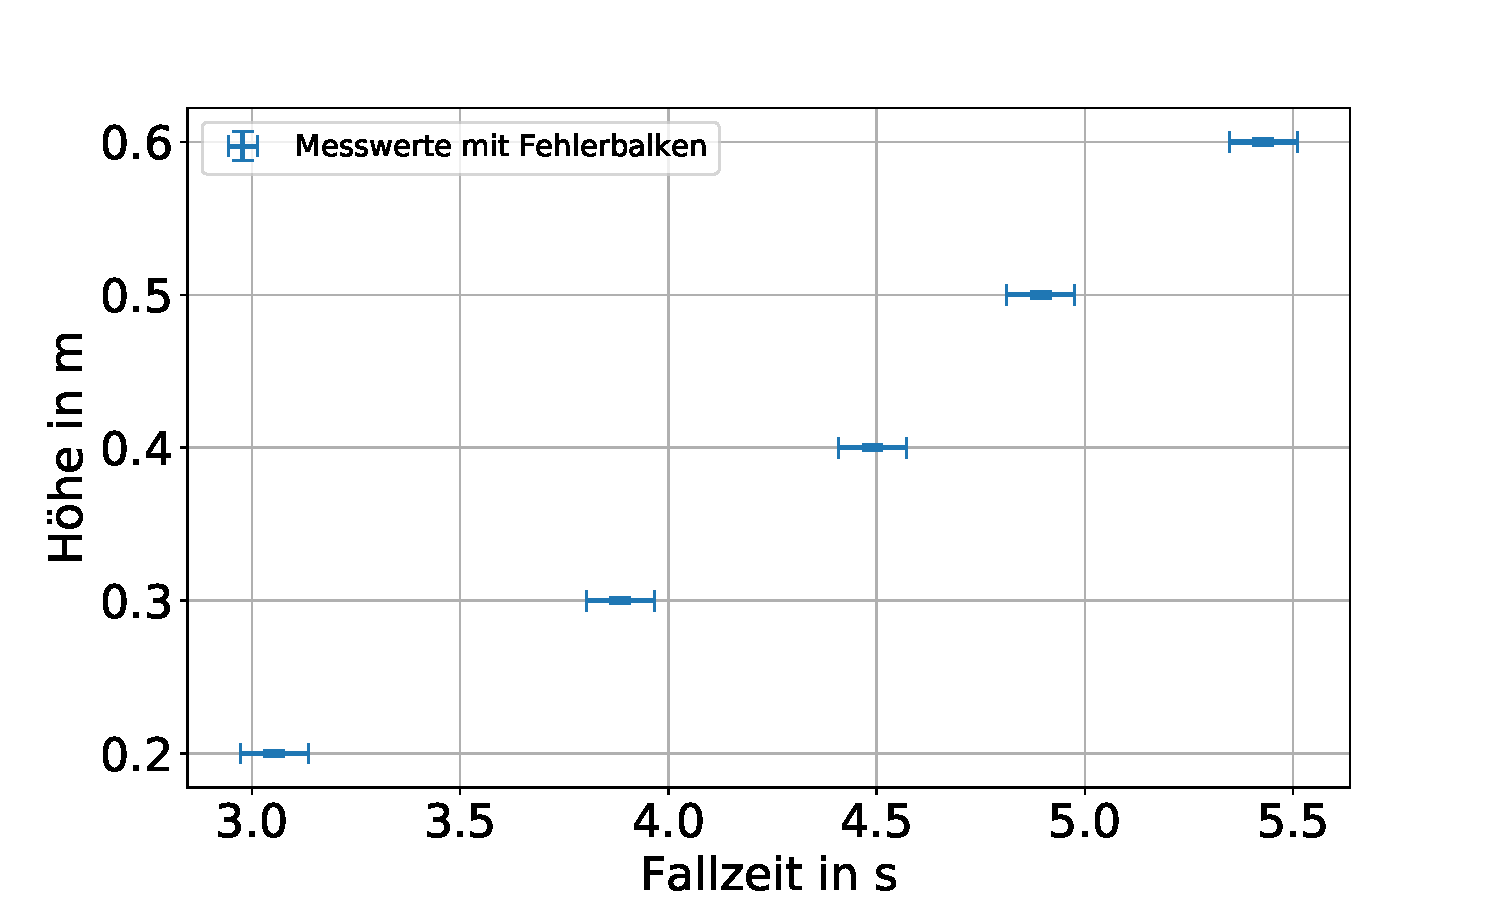
\includegraphics[width=0.7\linewidth]{auswertung/Fallrad/h,t}
	\caption{Die Höhe $h$ des Fallrades in Abhängigkeit der jeweiligen Fallzeiten $t$.}
	\label{fig:ht}
\end{figure}



\begin{figure}[h!]
	\centering
	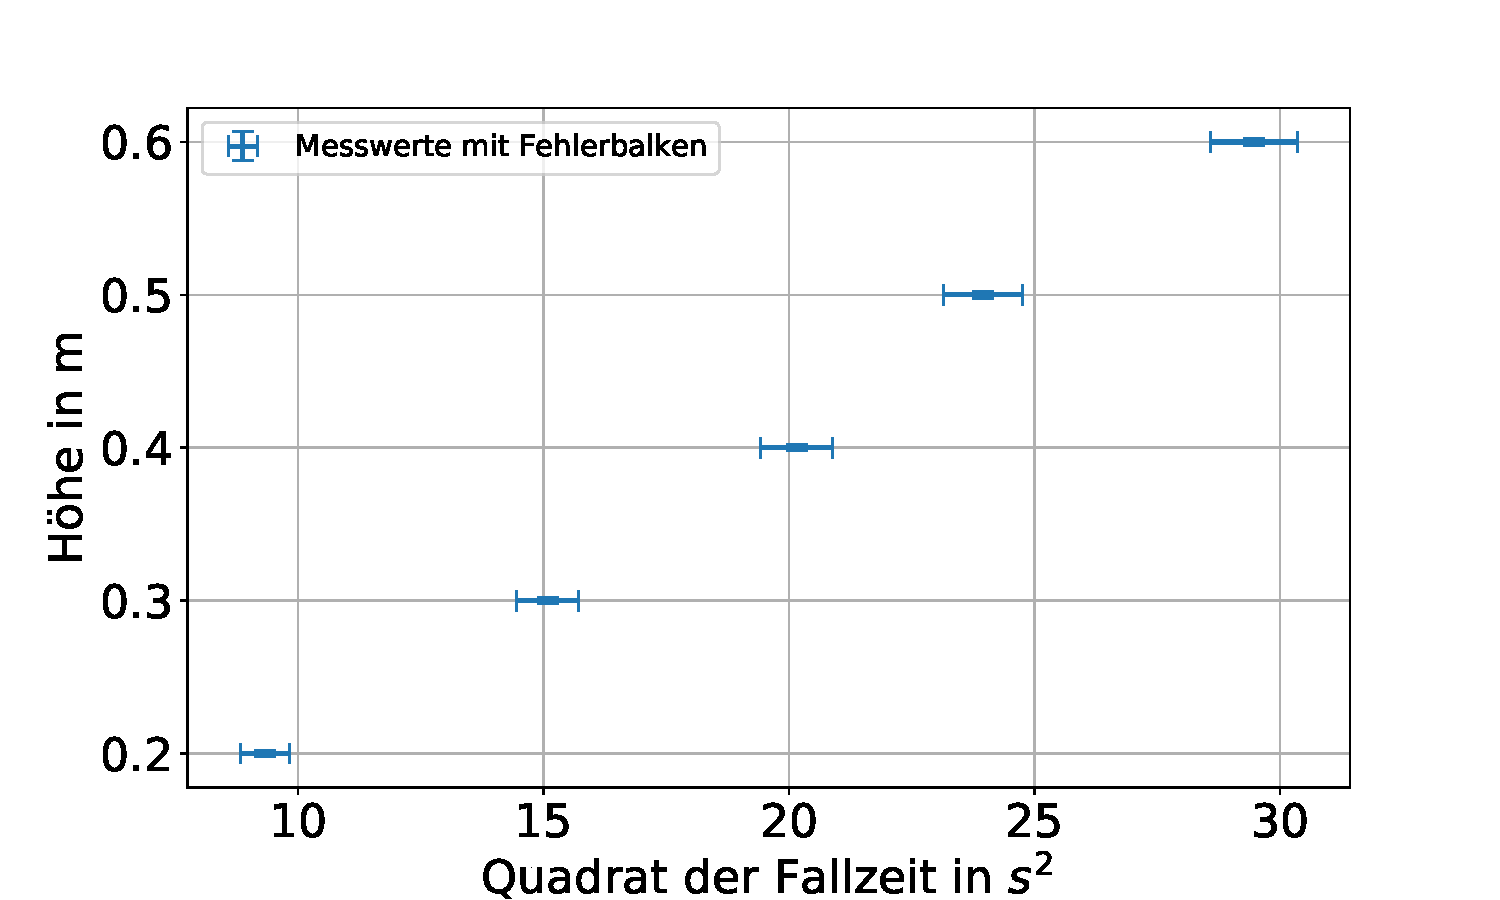
\includegraphics[width=0.7\linewidth]{auswertung/Fallrad/h,t^2}
	\caption{Die Messpunkte nach \cref{fig:ht} in Einheiten von $t^2$. }
	\label{fig:ht2}
\end{figure}

\begin{figure}[h!]
	\centering
	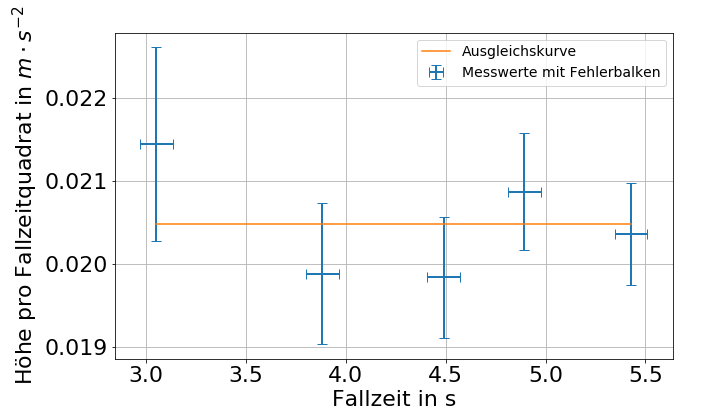
\includegraphics[width=0.7\linewidth]{auswertung/Fallrad/T,ht^-2}
	\caption{Messpunkte aus \cref{fig:ht} in Einheiten von $\frac{h}{t^2}$}
	\label{fig:tht-2}
\end{figure}





Die Abbildung \ref{fig:ht} stellt die Messwerte dar. Da die theoretischen Betrachtungen und der Graph eine quadratische Abhängigkeit suggerieren, werden diese Messwerte anschließend in Abbildung \ref{fig:ht2} linearisiert dargestellt. Abbildung \ref{fig:tht-2} stellt die jeweiligen Steigungen einer geraden durch Ursprung und Messpunkt der Abbildung \ref{fig:ht2} dar. \\






Anschließend wurde das arithmetische Mittel $c$ der Datenpunkte aus Abbildung \ref{fig:tht-2} gebildet. Aus der zugehörigen Bewegungsgleichung ist abzulesen, dass $\frac{g^*}{2}=\frac{h}{T^2}=c$. Es folgt: $g^*=\SI{0.0410 \pm  0.0019}{m \per s \squared}$.





\subsubsection{Vergleich der Abrollradien}


Aus der Zusammenhang zwischen der effektiven Beschleunigung und  dem Abrollradius nach Gleichung \ref{eq:gs} folgt für den Abrollradius Gleichung \ref{eq:R}.

\begin{align}
g^*  &= g \frac{mR^2}{J_s + m R^2}= 2c \label{eq:gs}\\
R&=\sqrt{\frac{2 c J_s}{M (g-2c)}} \label{eq:R}
\end{align}

Mit den Messwerten aus Tabelle \ref{tab:datafall}, der effektiven Beschleunigung $g^*$ aus Abbildung \ref{fig:tht-2} sowie der Fallbeschleunigung g aufgrund des Erdschwerefeldes und der Unsicherheit nach Gleichung \ref{eq:uR} folgt $R=\SI{0.00460\pm 0.00011}{m}$. Die Messung der Durchmesser von Faden und Aufhängeachse mit dem Messschieber ergab einen Radius $R_{geometrisch}=\SI{0.00455 \pm 0.00004}{m}$. Der direkt gemessene Radius bestätigt den zuvor errechneten Wert. Des weiteren liefert die direkte Messung erwartungsgemäß die kleinere Unsicherheit.  